\documentclass[12pt,a4paper]{article}
\usepackage[UTF8]{ctex}     %先引入ctex
\usepackage[utf8]{inputenc} %再引入inputenc
\usepackage{graphicx}
\usepackage{geometry}
\usepackage{xcolor}
% \usepackage{lazylatex}
\usepackage{amsmath}
\usepackage{enumerate}
\usepackage{caption}
\usepackage{listings}
\captionsetup[lstlisting]{labelfont=bf,justification=justified}

\usepackage{tikz}
\usepackage{appendix}

\graphicspath{{img/}}
% 边距
\geometry{left=2.0cm,right=2.0cm,top=2.0cm,bottom=3.0cm}
% 大题
\newenvironment{problems}{\begin{list}{}{\renewcommand{\makelabel}[1]{\textbf{##1}\hfil}}}{\end{list}}
% 小题
\newenvironment{steps}{\begin{list}{}{\renewcommand{\makelabel}[1]{##1.\hfil}}}{\end{list}}
% 答
\providecommand{\ans}{\textbf{答}:~}
% 解
\providecommand{\sol}{\textbf{解}.~}

\usepackage[colorlinks,linkcolor=blue]{hyperref}
\usepackage{bookmark}
\providecommand{\code}[2]{\lstinputlisting[language=#2,caption=\href{run:#1}{\ttfamily #1}]{#1}}
\providecommand{\img}[1]{\includegraphics[width=0.88\textwidth]{#1}}

% listings
\definecolor{grey}{rgb}{0.8,0.8,0.8}
\definecolor{darkgreen}{rgb}{0,0.3,0}
\definecolor{darkblue}{rgb}{0,0,0.3}
\lstset{%
    % numbers=left, %行号
    % numberstyle=\tiny\color{grey},
    showstringspaces=false,
    showspaces=false,%
    tabsize=4,%
    frame=shadowbox,%
    basicstyle={\ttfamily\scriptsize},%
    keywordstyle=\color{blue!80!black}\bfseries,%
    identifierstyle=,%
    commentstyle=\color{green!50!blue}\itshape,%
    stringstyle=\color{green!50!black},%
    rulesepcolor=\color{gray!20!white},
    breaklines,
    columns=flexible,
    extendedchars=false,
    %mathescape=true,
}

\begin{document}
\title{\normalsize \underline{操作系统(D)}\\\LARGE 项目 2}
\author{Log Creative }
\date{\today}
\maketitle

\begin{problems}
    \item[一] \textbf{Unix 外壳程序}
    \begin{steps}
        
        \item[1] 在子进程中执行命令
        
        \img{ps.png}

        同时执行命令:

        \img{psc.png}

        当输入 \verb"exit" 时,会退出外壳程序:

        \img{exit.png}

        可以看到外壳主进程在子进程尚未打印完成前就已经开始等待用户输入了,也就是两个进程同时进行。

        该部分需要获取用户输入,这里采用了 \texttt{fgets} 函数获取用户的整行输入。
        \begin{lstlisting}[language=c]
            fgets(rline, MAX_LINE, stdin);
        \end{lstlisting}
        第二参数用于说明最大读入字符数,将会限定最大的范围防止越界。该函数也支援存储换行符 \verb"\n"。

        在遍历输入字符时,如果遇到 \verb"&" 字符,将会对 \verb"should_wait" 标志置为 0,
        \begin{lstlisting}[language=c]
            case '&':
                should_wait = 0;
        \end{lstlisting}
        在之后的子进程创建函数中将会根据这个标志判定是否等待:
        \begin{lstlisting}[language=c]
            pid_t pid;
            pid = fork();

            if (pid < 0) fprintf(stderr, "Fork Failed"); 
            else if (pid == 0) return execvp(args[0],args);
            else if (should_wait) wait(NULL);
        \end{lstlisting}

        对于 \verb"args" 数组的存储,将会将每个字符串数组的起始位置指向 \verb"rline" 用户输入数组的对应位置(该过程通过判定前一个字符是否是空格实现),以实现参数存储
        \begin{lstlisting}[language=c]
            default:
                if (prev == ' ') args[argc++] = rptr;
                prev = *rptr;
                break;
        \end{lstlisting}
        
        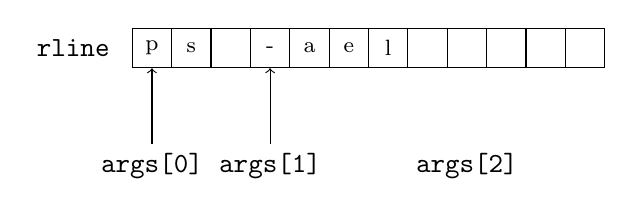
\begin{tikzpicture}
\tikzstyle{box} = [minimum width=0.5cm, minimum height=0.5cm, draw, font=\footnotesize];

\foreach \x/\y in {1/p,2/s,3/,4/-,5/a,6/e,7/l,8/,9/,10/,11/,12/}
	\node[box] (n-\x) at (\x*0.5,0) {\y};

\node at (-0.5,0) {\texttt{rline}};
\node (t-0) at (0.5,-1.5) {\verb"args[0]"};
\draw[->] (t-0) edge (n-1);
\node (t-1) at (2,-1.5) {\verb"args[1]"};
\draw[->] (t-1) edge (n-4);
\node at (4.5,-1.5) {\verb"args[2]"};
\end{tikzpicture}


        当遇到空格、换行、\verb"&"符号时,都会被替换为 \verb"\0",从而限制每一个字符串数组的终止位置,读到换行符会强制终止循环
        \begin{lstlisting}[language=c]
            case '&':
                should_wait = 0;
            case '\n':
                flag = 1;
            case ' ':
                prev = *rptr;
                *rptr = '\0';
                break;
        \end{lstlisting}

        最后一个参数根据规定,必须被赋值为空指针
        \begin{lstlisting}[language=c]
            args[argc] = NULL;
        \end{lstlisting}

        退出的判定是通过 \verb"strcmp" 函数实现的
        \begin{lstlisting}[language=c]
            should_run = strcmp(args[0],"exit");
        \end{lstlisting}

        \item[2] 历史记录存储
        
        当输入 \verb"!!" 时将会回显并运行上一条指令

        \img{history.png}

        当没有上一条指令时,将会返回提示

        \img{nohist.png}

        这一部分需要将上一条指令存储在 \texttt{buf} 中,开始时置为空
        \begin{lstlisting}[language=c]
            char buf[MAX_LINE] = "\0";
        \end{lstlisting}

        当连续输入两个 \verb"!" 时,将会首先检查 \verb"buf[0]" 是否是空字符,否则将通过 \verb"memcpy" 将缓存复制到当前的阅读行数组中,注意这里不能使用 \verb"strcpy",因为其的复制到 \verb"\0" 就会立刻停止,导致后面的部分没有被有效复制。如果是其他指令,则会被存储到缓冲区中去。
        \begin{lstlisting}[language=c]
            if (strcmp(rline,"!!\n")==0){
                if(!buf[0]){
                    fprintf(stdout, "%s\n", "No commands in history.");
                    flag = -1;
                } else {
                    memcpy(rline, buf, MAX_LINE*sizeof(char));
                    fprintf(stdout, "%s", rline);
                }
            } else memcpy(buf, rline, MAX_LINE*sizeof(char));
        \end{lstlisting}

        如果不是正常指令,将不会执行任何指令。
        \begin{lstlisting}[language=c]
            if(flag == -1) continue;
        \end{lstlisting}

        \item[3] 重定向输入输出
        
        \verb"in.txt" 里面存有一些乱序的数字
        \code{src/in.txt}{}

        \img{redir.png}

        \verb"out.txt" 的文件将命令的输出存储。
        \code{src/out.txt}{}

        首先需要识别输入输出符号
        \begin{lstlisting}[language=c]
            case '>':
                file_mode = O_WRONLY;
                args[argc++] = NULL;
                prev = ' ';
                file_arg = argc;
                break;
            case '<':
                file_mode = O_RDONLY;
                args[argc++] = NULL;
                prev = ' ';
                file_arg = argc;
                break;
        \end{lstlisting}
        其中 \verb"file_mode" 存储打开文件的模式:\verb"O_WRONLY" 以只写方式打开文件,等价为 1;\verb"O_RDONLY" 以只读方式打开文件,等价为 0。\verb"file_arg" 存储文件名的位置,便于后续调用。而作为命令而言,命令应当在输入输出符号之前终结,因此这里需要添加示意终结的符号 \verb"NULL";并且将输入输出符号识别为分隔符号,令为空格。

        当识别文件模式大于等于 0 时,就会在子进程中截获控制台输入与输出。在写入模式下,如果文件不存在,文件会被创建。值得一提的是,使用 \verb"dup2" 截获子进程的控制台输入输出并不会影响主进程的输入输出,所以就没有必要去使用一个变量存储主进程的输入输出文件描述符,再赋值回去。子进程需要在完成使用后关闭文件。
        \begin{lstlisting}[language=c]
            // child process
            if(file_mode >= 0){
                fd = open(args[file_arg], file_mode, PERMS);
                if(file_mode == O_WRONLY){
                    if(fd == -1) fd = creat(args[file_arg], PERMS);
                    if(fd == -1) fprintf(stderr, "%s %s.\n", "Cannot write file", args[file_arg]);
                    else dup2(fd, STDOUT_FILENO);
                } else if (file_mode == O_RDONLY){
                    if(fd == -1) fprintf(stderr, "%s %s.\n", "Cannot read file",args[file_arg]);
                    else dup2(fd, STDIN_FILENO);
                }
            }
            execvp(args[0],args);
            if(fd != -1) close(fd);
            return 0;
        \end{lstlisting}
        其中 \verb"PERMS" 被定义为对于所有者、所有者组和其他成员均可读写。
        \begin{lstlisting}[language=c]
            #define PERMS 0666
        \end{lstlisting}

        \item[4] 通过管道建立通信
        
        输入管道命令

        \img{less.png}

        可以看到数值被正确传入了后一个命令中。
        
        \img{pipe.png}

        首先仍然是识别管道符号:
        \begin{lstlisting}[language=c]
            case '|':
                args[argc++] = NULL;
                prev = ' ';
                pipe_arg = argc;
                break;
        \end{lstlisting}
        其中 \verb"pipe_arg" 将会存储管道命令开始的位置,当其不为小于 0 的值时,将会触发子进程再次新建一个子进程,并通过管道连接两者。
        \begin{lstlisting}[language=c]
            if(pipe_arg < 0){
                // original child commands ...
            } else {
                int pfd[2];
                pid_t ppid;

                if (pipe(pfd) == -1){
                    fprintf(stderr, "Pipe Failed");
                    continue;
                }

                ppid = fork();

                if(ppid < 0){
                    fprintf(stderr, "Child Fork Failed");
                    continue;
                }

                if(ppid > 0){
                    close(pfd[READ_END]);
                    dup2(pfd[WRITE_END], STDOUT_FILENO);
                    execvp(args[0],args);
                    close(pfd[WRITE_END]);
                } else {
                    close(pfd[WRITE_END]);
                    dup2(pfd[READ_END], STDIN_FILENO);
                    execvp(args[pipe_arg],&args[pipe_arg]);
                    close(pfd[READ_END]);
                }
            }
        \end{lstlisting}
        子进程将前一个命令的输出输入管道的写入端,子子进程将管道端的读入部分作为自己的输入。这样就完成了管道通信。

        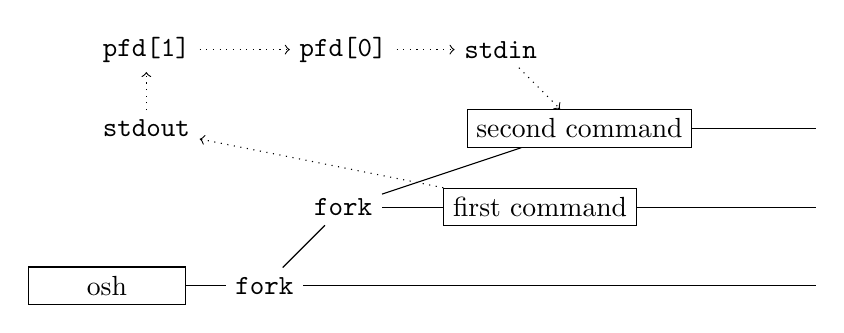
\begin{tikzpicture}
\tikzstyle{process} = [minimum width=2cm,draw,];
\tikzstyle{thread} = [minimum width=2cm,draw,dashed]
\tikzstyle{message} = [->,dotted];

\node [process] (v1) at (-3.5,0) {osh};
\node [process] (v2) at (2,1) {first command};
\node [process] (v5) at (2.5,2) {second command};

\node (v3) at (-1.5,0) {\texttt{fork}};
\draw  (v1) edge (v3);
%\draw  (v3) edge (v2);
\node (v4) at (-0.5,1) {\texttt{fork}};
%\draw  (v2) edge (v4);
\draw  (v4) edge (v5);
\draw (v3) -> (5.5,0);
%\draw (v4) -> (3,1);
\draw (v5) -> (5.5,2);
\node (v7) at (-3,3) {\texttt{pfd[1]}};
\node (v6) at (-3,2) {\texttt{stdout}};
\node (v8) at (-0.5,3) {\texttt{pfd[0]}};
\node (v9) at (1.5,3) {\texttt{stdin}};
\draw [message] (v2) edge (v6);
\draw [message] (v6) edge (v7);
\draw [message] (v7) edge (v8);
\draw [message] (v8) edge (v9);
\draw [message] (v9) edge (v5);
\draw  (v3) edge (v4);
\draw  (v4) edge (v2);
\draw (v2) -- (5.5,1);
\end{tikzpicture}
        
    \end{steps} 
    
    \item[二] \textbf{任务信息内核模块}
    
    安装模块 \verb"pid" 后,将进程号输入文件,读取时将会展示进程的相关信息。

    \img{pid.png}

    \begin{steps}
        \item[1] 写入文件
        
        读取到用户信息后,使用 \verb"sscanf" 获取变量并赋值到模块变量 \verb"l_pid" 中。
        \begin{lstlisting}[language=c]
            sscanf(k_mem,"%ld",&l_pid);
        \end{lstlisting}

        \item[2] 读取文件 
        
        当获取到 \verb"tsk" 变量时,将会返回进程的相关信息,通过 \verb"sprintf" 读取到 \verb"buffer" 中,稍后将会被返回到用户区,注意此处需要暂存返回的字符串长度到变量 \verb"kv" 中以便返回用户区时系统知晓需要读取的字符数。

        \begin{lstlisting}[language=c]
            if(tsk!=NULL)
                rv = sprintf(buffer,"command = [%s] pid = [%ld] state = [%ld]\n",tsk->comm,l_pid,tsk->state);
            else 
                rv = sprintf(buffer,"pid [%ld] is not found!\n",l_pid);
        \end{lstlisting}

    \end{steps}

\end{problems}

\begin{appendix}
    \section{全部代码}

    \code{src/Makefile}{}
        
    \code{src/osh.c}{c}

    \code{src/pid.c}{c}

\end{appendix}

\end{document}
